%! TEX root = ../main.tex
\documentclass[../main.tex]{subfiles}
\begin{document}

% ============================================================ %
% ============================================================ %
\chapter{ML design}
% ============================================================ %
% ============================================================ %

\section{Principles}
\subsection{Characteristics of ML systems}
There are key differences between Machine Learning during the training phase and during the prediction phase.
By design, these 2 phases will face different challenges. So the systems will be designed very differently.
\textbf{But code should be shared between the 2 phases to avoid model misuse.}
\begin{center}
    \begin{tabular}{ |c|c|}
        \hline
        Phase & Key aspects \\
        \hline
        Training & Offline, model agnostic, iteration speed \\
        \hline
        Prediction & Real-time, production systems, scale, observability \\
        \hline
    \end{tabular}

\end{center}

\section{Challenges}
This section is a summary of \cite{tech-debt}.

\subsection{Complex models erode boundaries}
\begin{center}
    \begin{tabular}{ |c|p{10cm}|}
        \hline
        Challenge & Defintion \\
        \hline
        \hline
        Entanglement & ML systems mix signals together. Isolated improvements are impossible. \\
                     & CACE: Changing Anything Changes Everything \\
        \hline
        Correction Cascade & When chaining models, we create dependencies (e.g. multiple heads). \\
                           & This can create an improvement deadlock: improving any component leads to
                           system-level detriments. \\
        \hline
        Undeclared consumers & Creates hidden tight coupling of model to other parts of the stack.
            Changes to the model will impact other parts of the stack in unintended ways.
            This increases the cost and difficulty of making any changes to the model. \\
        \hline
    \end{tabular}
\end{center}

\subsection{Data dependencies cost more than code dependencies}

\subsubsection{Unstable data dependencies}
 Input signal may not be stable: output of other ML model that could
be updated, data-dependent look-up table. Also, owner of the input signal may decide to change
it. To mitigate, create a versioned copy of the input signal, e.g. freeze the input mapping, model
and use it until all consumers have upgraded to the new input. \\

\subsubsection{Underutilized data dependencies}
These are input signals that provide very little value
but by using them, the model is vulnerable to their change, whereas they could be remove
without detriment
\begin{center}
    \begin{tabular}{ |c|p{10cm}|}
        \hline
        Features type & Defintion \\
        \hline
        \hline
        Legacy features & Feature is included early in development, but is later made redundant. \\
        \hline
        Bundled features & A group of features is evaluated and found to be benefitial. All features
            are included without verifying if they are all relevant. \\
        \hline
        $\epsilon$-features & Feature that adds very little improvement (i.e. benchmark hacking) \\
        \hline
        Correlated features & 2 features are strongly correlated, but ML model won't understand it.
            This results in brittleness if the correlation later changes.\\
        \hline
    \end{tabular}
\end{center}

Underutilized features can be detected via exhaustive leave-one-feature-out evaluations. These should
be run regularly to identify and remove unnecessary features.

\subsection{Feedback loops}
\subsubsection{Direct feedback loop}
A model may directly influence the selection of its own future training data.

\subsubsection{Hidden feedback loop}
When 2 systems influence each other indirectly. E.g. 2 models defining the items to show in a Web
page. Changing one model will change the user's behaviour, which is most likely one input signal
to the 2nd model. \\
Other example, competing models on the stock market. Any modification of one model will change the
behaviour of the competing models as a consequence. Note that the introduced modification could be
a bug.

\subsection{ML-system anti-patterns}
\subsubsection{Glue code}
95\% of the code in a mature ML system is glue code, 5\% is machine learning code. Glue code is costly
in the long term because it tends to freeze a system to the peculiarities of a specific package. Testing
alternatives may become prohibitively expensive. \\
A common strategy for combating glue code is to wrap black-box packages into common APIs.

\subsubsection{Pipeline jungles}
Often appears in data preparation, these can evolve organically, as new signals are identified and new
sources added incrementally. Without care, the system may become a jungle of scrapes, joins and sampling steps
, often with intermediate files output. Detecting errors and recovering from failures will be difficult
and costly, \\
Avoid by thinking holistically baout data collection and features extraction. Scraping and redesigning
a pipeline jungle is a major investment, but it can dramatically reduce ongoing costs and speed further
innovation.

\subsubsection{Dead experimental codepaths}
As a consequence of glue code and pipeline jungles, it becomes attractive in the short term to
experiment alternative methods by implementing experimental codepaths as conditional branches within
the main production code. Over time, these accumulated paths create a growing debt due to the increasing
difficulty of maintaining backward compatibility and exponential cyclomatic complexity.\\
Avoid by periodically re-examining the experimental branch and remove the unused ones.

\subsubsection{Abstraction debt}
Due to a lack of strong abstractions in ML, it is too easy to blur the line between the components.

\subsubsection{Common smells}
\begin{center}
    \begin{tabular}{ |c|p{10cm}|}
        \hline
        Smell & Definition \\
        \hline
        \hline
        Plain-old-data type smell& ML outputs do not come with metadata to explain their nature.
            E.g.: is that p(x) or 1-p(x)? Is this a log?  \\
        \hline
        Multiple-language smell & Using multiple languages increases the cost of effective testing
            and increases difficulty of transferring ownership to other individuals.\\
        \hline
        Prototype smell & The project relies on a protoyping environment. Full-scale system may be
            brittle, difficult to change. In times of pressure, this prototyping environment will be
            pushed to production. What's more, results at small scale rarely reflect reality at
            full scale.\\
        \hline
    \end{tabular}
\end{center}

\subsection{Fighting configuration debt}
ML systems come with many parameters that can be configured. Input signals may be changed, composed
out of many input signals that may also change, or be disabled. As a result, signals are created from
complex rules that are hard to track. \\
To limit configuration debt, follow these principles:
\begin{itemize}
    \item It should be easy to specify a configuration as a small change from a previous configuration.
    \item It should be hard to make manual errors, omissions or oversights.
    \item It should be easy to see, visually, the difference in configuration between 2 models.
    \item It should be easy to automatically assert and verify basic facts about the configuration:
        number of features used, transitive closure of data dependencies, ...
    \item Configurations should undergo a full code review and be checked into a repository.
\end{itemize}

\subsection{Dealing with changes in the external world}
\subsubsection{Fixed thresholds in dynamic systems}
It is often needed to pick a \textbf{decision threshold}. Usually it is manually selected to
obtain a good trade-off out of a list of thresholds. When input data changes, the threshold may be
obsolete.\\
To mitigate the problem, we can regurlarly tune the thresholds on held out validation data.

\subsubsection{Monitoring and testing}
Comprehensive live monitoring of system behavior in real time combined with automated response
is critical for long-term system reliability.
Following points should be monitored:
\begin{itemize}
    \item \textbf{Prediction bias} Verify that the prediction distribution is stable. Changes in this
        metrics are often indicative of input data changes. Slicing prediction bias isolate issues quickly,
        and can be used for automated alerting.
    \item \textbf{Action limits} When the system can take actions, we can enforce action limits as a sanity
        check. These limits should be broad enough not to trigger spuriously.
    \item \textbf{Up-stream producers} Up-stream processes should be thoroughly monitored, tested and
        routinely meet a service-level objective that takes the downstream ML system needs into account.
        Any up-stream alerts must be propagated to the control pane of the ML system to ensure its
        accuracy.
\end{itemize}

\subsection{Other areas of ML-related debt}
\subsubsection{Data testing debt}
Testing input data is critical to a well-functioning system. It can be basic sanity check or more
sophisticated tests that monitor changes in input distribution.

\subsubsection{Reproducibility debt}
As scientists, it is important we can re-run experiments and get similar results. But in the case
of real-world systems, it is difficult.

\subsubsection{Process management debt}
Mature systems contain dozens or hundreds of models running simultaneously. This raises a wide range
of important problems, such as updating many configurations safely and automatically, managing and assigning
resources among models, how to visualize and detect blockages in the flow of data. Developing tooling
to aid recovery from production incidents is also critical. \textbf{An important system-level smell
to avoid is common processes with many manual steps.}

\subsubsection{Cultural debt}
Research and development goes together. It is important to create team cultures that reward deletion
of features, reduction of complexity, improvements in reproducibility, stability, and monitoring to the
same degree that improvements in accuracy are valued.

\subsection{Conclusion: measuring debt and paying it off}
Measuring debt is complicated, a few useful questions to consider are:
\begin{itemize}
    \item How easy can an entirely new algorithmic approach be tested at full scale?
    \item What is the transitive closure of all data dependencies?
    \item How precisely can the impact of a new change to the system be measured?
    \item Does improving one model or signal degrade others?
    \item How quickly can new members of the team be brought up to speed?
\end{itemize}
\\
The paper sums it up extremely well:
\begin{displayquote}
    \enquote{Paying down ML-related technical debt requires a specific commitment, which can often only
        be achieved by \textbf{a shift in team culture}. Recognizing, prioritizing, and rewarding this
        effort is important for the long term health of successful ML teams.}
\end{displayquote}

\end{document}

\section{Systems design interview}
\subsection{Requirements clarification}
Ask clarification questions to the interviewer, this shows how you handle ambiguity. The interviewer
is also starting to gauge your seniority level. There are 4 main axes for requirements to clarify:
\begin{center}
    \begin{tabular}{ |c|p{10cm}|}
        \hline
        Users / Customers & Who will use the system? How will it be used?\\
        \hline
        Scale (read \& write) & How many read queries per second?
            How much data is queried per request? Can there be spikes in the traffic?  \\
        \hline
        Performance & Expected write-to-read data delay? Expected p99 latency for read?\\
        \hline
        Cost & Should we minimize development cost? Maintenance cost?\\
        \hline
    \end{tabular}
\end{center}

There are 2 types of requirements: \textbf{functional} requirements are the definitions of the API and
what it will do. \textbf{Non-functional} requirements are system qualities: fast, fault-tolerant,
secure... \\
For functional requirements, phrase with simple sentences what the system should do. Then, start iterating
over the very key API endpoints (e.g. \verb|countViewEvent(videoId)| $\to$
\verb|coutEvent(videoId, eventType)|, ...). This helps identify names of APIs, input parameters.\\
For non-functional requirements,

\subsection{High-level architecture}
Start with describing the system with high-level components (e.g. DB, processing service, query service...).
Interviewer will be an expert in the field, so he will have questions already. To avoid being drown in
questions, we have to drive the discussion. So where to start? Start with the \textbf{outside pieces}:
\textbf{the data}. We have to define a data model.
\subsubsection{Data model}
First, deifne \textbf{what we store}. This directly leads to questions like: should I store raw data
or aggregated data? There are pros \& cons for each approach, and we should discuss them. \\

\paragraph{Where do we store the data?}
We need to evaluate DB systems against non-functional requirements: scalability, performance and
availability:
\begin{itemize}
    \item How to scale \textbf{reads} and \textbf{writes} ?
    \item How to make both \textbf{reads} and \textbf{writes} fast?
    \item How \textbf{not to lose data} in case of hardware faults and network partitions?
    \item How to achieve \textbf{strong consistency}? What are the trade-offs? (CAP theorem)
    \item How to \textbf{recover data} in case of an outage?
    \item How to ensure \textbf{data security}?
    \item How to make it \textbf{extensible} for data model changes in the future?
    \item Where to run (cloud VS on-premises data centers)?
    \item How much money will it cost?
\end{itemize}

\paragraph{How do we store the data?}
In SQL we think in terms of nouns: we define the tables from the nouns of entities. In NoSQL, we think
in terms of queries that will be executed. \\
There are 4 types of NoSQL databases: column, document, key-value and graph. \\

\subsection{Data aggregation basics}
\paragraph{Should we pre-aggregate data in the processing service?} Doing so allows us to limit the
number of queries to the DB. Processing service may push to DB every 1 or 2 seconds only. Data is
in-memory so R/W is very fast.\\

\paragraph{Push or pull?}
Pre-aggregation can create data loss, as the processing service contains some state. \textbf{Push}
means that we push data to the processing service. \textbf{Pull} means that we pull data from some
source (e.g. a message queue). If processing machine crashes we may still have events in the source.

\paragraph{Checkpointing}
Events are stored sequentially in the queue. This allows to define an offset. Instead of dumping the
message after a read, we simply increment the offset. When an offset limit is reached, we will sync
in-memory with the DB, dump read messages, and reset the offset. That way in case of crash,
a new machine can just start processing from the MQ as is (default state: offset=0).

\paragraph{Partitioning}
Use a hash based on input data to identify the queue to push the message to. That way, each processing
machine will process the events for specific elements and we will avoid maintaining a very large
in-memory state. This allows us to parallelize events processing.

\begin{figure}
    \centering
    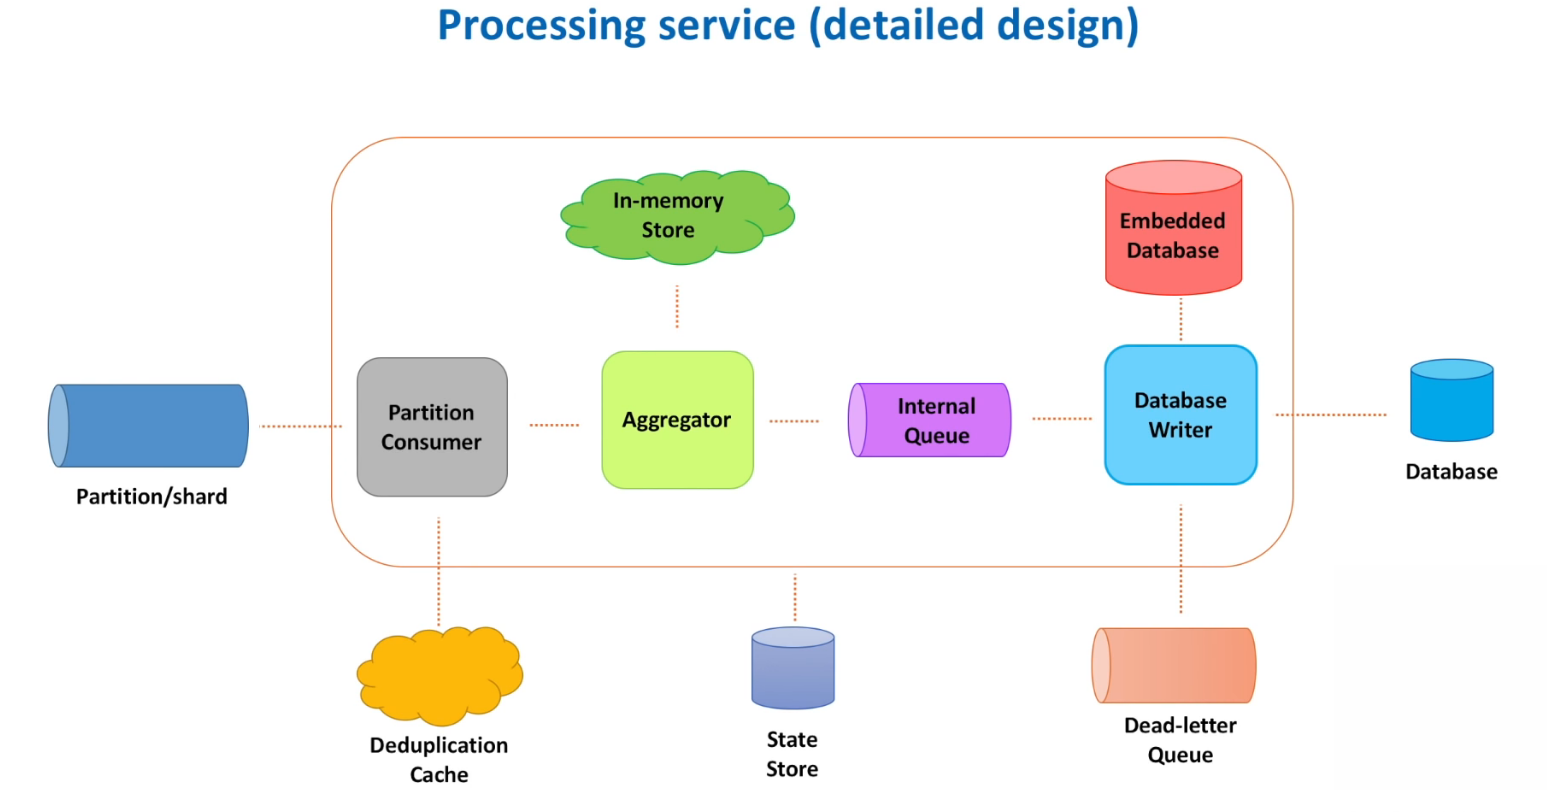
\includegraphics[width=12cm]{assets/processing-service.png}
    \caption{Processing service detailed design \cite{sys-design-interview-yt}}
\end{figure}

\subsection{Data ingestion path}
\begin{figure}
    \centering
    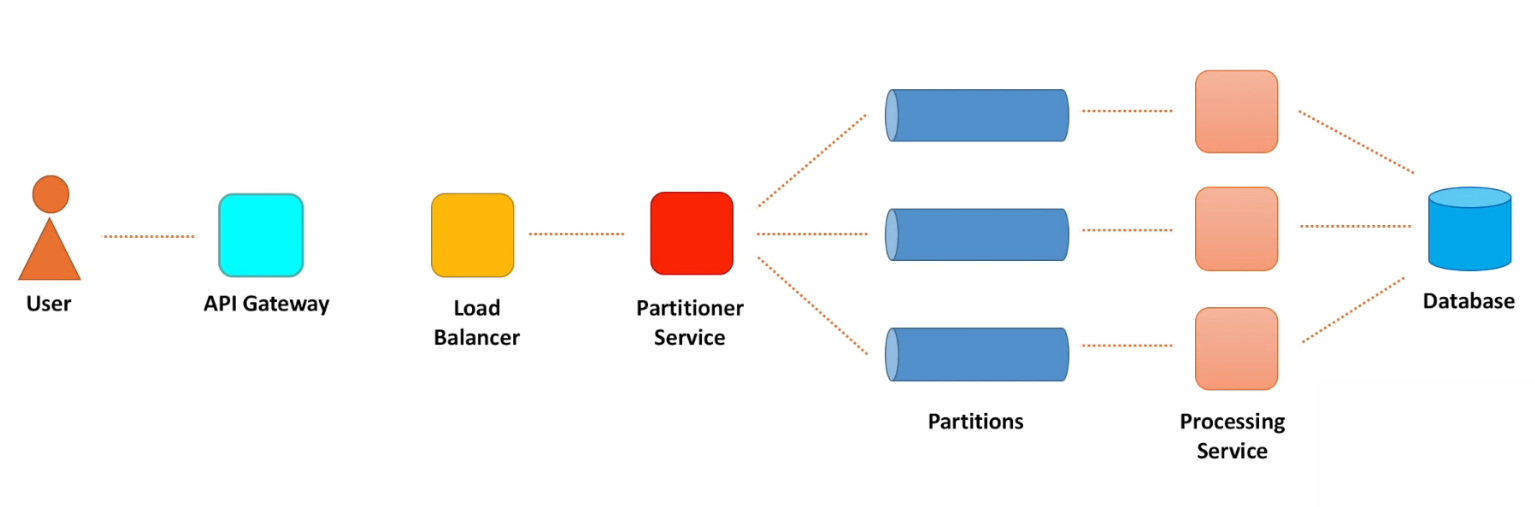
\includegraphics[width=12cm]{assets/ingestion-path.png}
    \caption{Ingestion path \cite{sys-design-interview-yt}}
\end{figure}

\subsubsection{Partitioner service client}
\paragraph{Blocking VS non-blocking I/O}
Blocking = 1 thread per request. Non-blocking = 1 thread for multiple requests. Non-blocking increases complexity, blocking system is easy to debug. We can track progress by looking in to the thread stack. Exceptions
pop up the stack and it is easy to catch and handle them. We can use thread local variables.

\paragraph{Buffering and batching}
Combine events into batches that are sent altogether to the partitioner service. But this introduces
complexity, e.g. when some events fail within a batch.

\paragraph{Timeouts}
Request timouts happens when request processing takes too much time, and client is not willing to wait
any longer. To choose the timeout value, analyze percentiles $\to$ how many \% of the requests will
time out?

\paragraph{Retries}
Retry when timed out, choose a different machine in case the original was faulty. To avoid overloading
the machines, use \textbf{exponential backoff} and \textbf{jitter}. Exponential backoff means waiting
more time with every retry, jitter adds randomness to spread out the load.

\paragraph{Circuit breaker}
Stops a client from repeatedly requesting. Simply calculate how many requests have failed recently
and if threshold is exceeded we stop calling a downstream service. This adds complexity and makes
debugging harder.

\subsubsection{Load balancer}
Distributes data traffic between multiple servers.
\paragraph{Software VS hardware load balancing}
\textbf{Hardware load balancing}: powerful machines with many CPUs, memory, optimized to handle millions
of requests per second. \textbf{Software load balancing}: software we install on any machine to do
load balancing.

\paragraph{Networking protocols}
\textbf{TCP} load balancers just forward the requests to the right machine $\to$ millions of request
per second. \textbf{HTTP} load balancers can look inside the message and make a decision based on the
content (e.g. cookie or header).

\paragraph{Load balancing algorithms}
Round robin sends connection in order to the list of servers. We can also use least connections or
least response time. We can also use hash-based algorithm.

\paragraph{Domain Name System}
We need to register our partitioner service in DNS (e.g. part.domain.com). Requests are routed to the
load balancer, which needs to know the IP adresses of the partioner service machines. Load balancers
need to know which server is healthy $\to$ \textbf{health check}.

\paragraph{High availability}
There are primary and secondary load balancers. Primary nodes handle requests, secondary ones monitor
the primary ones. Secondary takes over in case the primary faces issues. Primary and secondary should
live in different data centers.

\subsubsection{Partitioner service and partitions}
\paragraph{Partition strategy}
We can hash some content of the request to define partitions. But we have to careful about
\textbf{hot partitions}. This happens when we hash based on unbalanced information, e.g. hash the video
ID, but some videos are viral. A solution can be to add the datetime of the request to the hashed information.
Another way is to split the hot partitions into 2 new partitions.

\paragraph{Service discovery}
\textbf{Server-side} discovery: load balancers do that for the partitioner service client.
\textbf{Client-side} discovery: the client talks directly to the service registry. This means less
network hops but the client must have knowledge of the service registry. Service registry may be
integrated inside the partition nodes, e.g. in Cassandra each node knows about all the other nodes.

\paragraph{Replication}
Replicate data to avoid losing it. There are multiple approaches: single leader, mutliple leader,
leaderless. \textbf{Single leader}: 1 leader, many followers. We read and write from the leader.
Followers replicate data and can take over when leader crashes. Leader monitors followers and update
the list of followers if needed.

\paragraph{Message formats}
Message can be textual (e.g. JSON, XML) or binary (e.g. ProtoBuf, Avro). Binary ones are smaller and
faster to parse. Binary formats can use tags (1, 2, 3) instead of names for fields. Using binary
messages means sharing the schemas between producers and consumers. Binary formats may not allow for
insertion of new fields.

\subsection{Data retrieval path}
For single value, there are not many problems. But for time-series that are ever expanding, storage
will explode even if we compile per minute. The solution is to rollup the data: 1 minute granularity for
1 week, 1 hour granularity for 1 month, 1 day granularity for 3 months, ... \\
Older data can be pushed to an object storage like S3 instead of in the DB. DB is the \textbf{hot storage},
S3 is the \textbf{cold storage}. We can even introduce a \textbf{distributed cache} to store query results
and retrieve them.


\begin{figure}
    \centering
    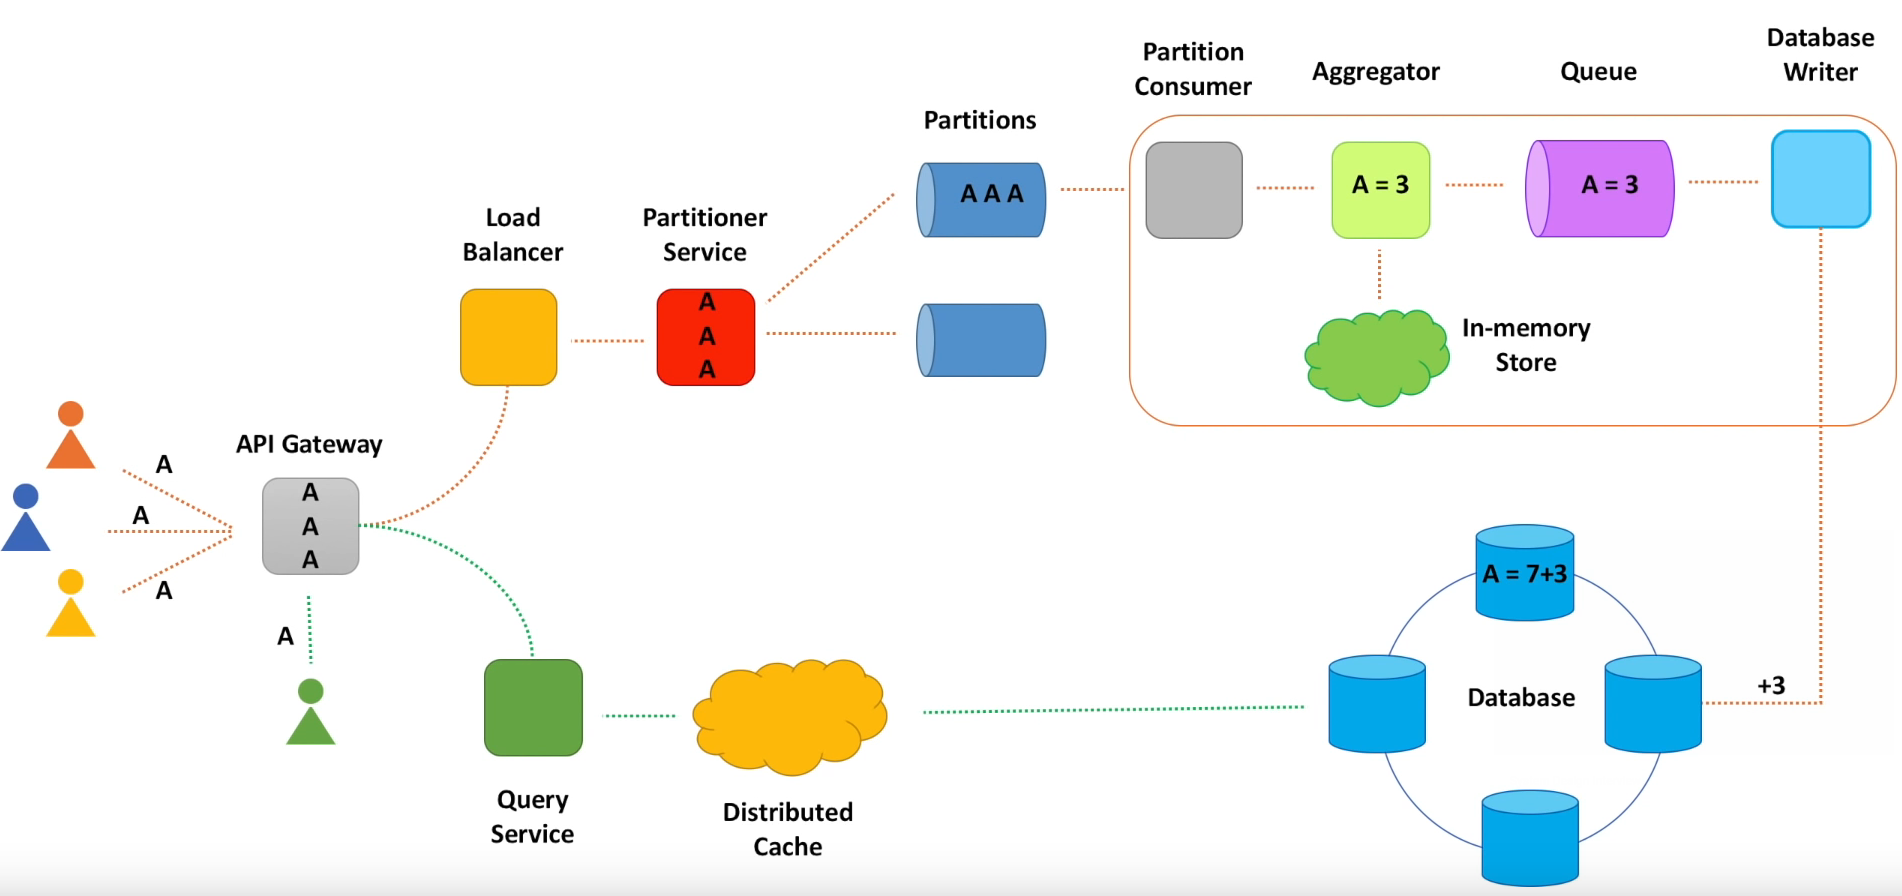
\includegraphics[width=12cm]{assets/data-flow.png}
    \caption{Full data flow path \cite{sys-design-interview-yt}}
\end{figure}

\subsection{Technology stack}
\begin{center}
    \begin{tabular}{ |c|p{10cm}|}
        \hline
        Load balancing & Citrix Netscaler (Hardware), NGINX, AWS ELB \\
        \hline
        Messaging systems & Apache Kafka, AWS Kinesis \\
        \hline
        Data processing & Apache Spark, Apache Flink, AWS Kinesis Data Analytics\\
        \hline
        Storage & Apache Cassandra, Apache HBase (time-series), Hadoop, Redshift, S3\\
        \hline
    \end{tabular}
\end{center}

\subsection{Bottlenecks and trade-offs}
\subsubsection{Identifying bottlenecks with performance testing}
\begin{table}[!htbp]
    \begin{tabular}{ |c|p{6cm}|p{6cm}|}
        \hline
        Test type & Set up & Learnings \\
        \hline
        \hline
        Load testing &
        Expose system to typical load &
        System is scalable  and can handle expected load, up to 2-3x \\
        \hline
        Stress testing &
        Increase load until it starts breaking apart &
        Which component will start to suffer first, and which resources it will be\\
        \hline
        Soak testing &
        Expose system to continuous load over a long period of time &
        Find leaks in resources\\
        \hline
    \end{tabular}
    \caption{Types of performance tests}
\end{table}

\subsubsection{Health monitoring}
Use metrics, dashboards and alerts. The 4 golden signals of monitoring are: \textbf{latency, traffic,
errors, and saturation}.

\subsubsection{Making sure the results are accurate}
We need an audit system, there are 2 types of audit systems. A \textbf{weak} audit system is a
continuously running E2E test (e,g, every minute perform a E2E test on the running system). This will
catch most errors, but rare bugs in rare scenarios will be hard to spot. A \textbf{strong} audit system
will compute results using a completely different path. This reminds of the Lamda architecture where
we have a stream processing system and a batch processing system in parallel.

\subsubsection{Making sure the load is spread out}
Use a smart partitioning to avoid having hot partitions.

\subsubsection{Handling too many messages}
We can batch incoming data and send a message whenever a new batch is ready. We obtain a hybrid system
between stream processing and batch processing.

\begin{figure}
    \centering
    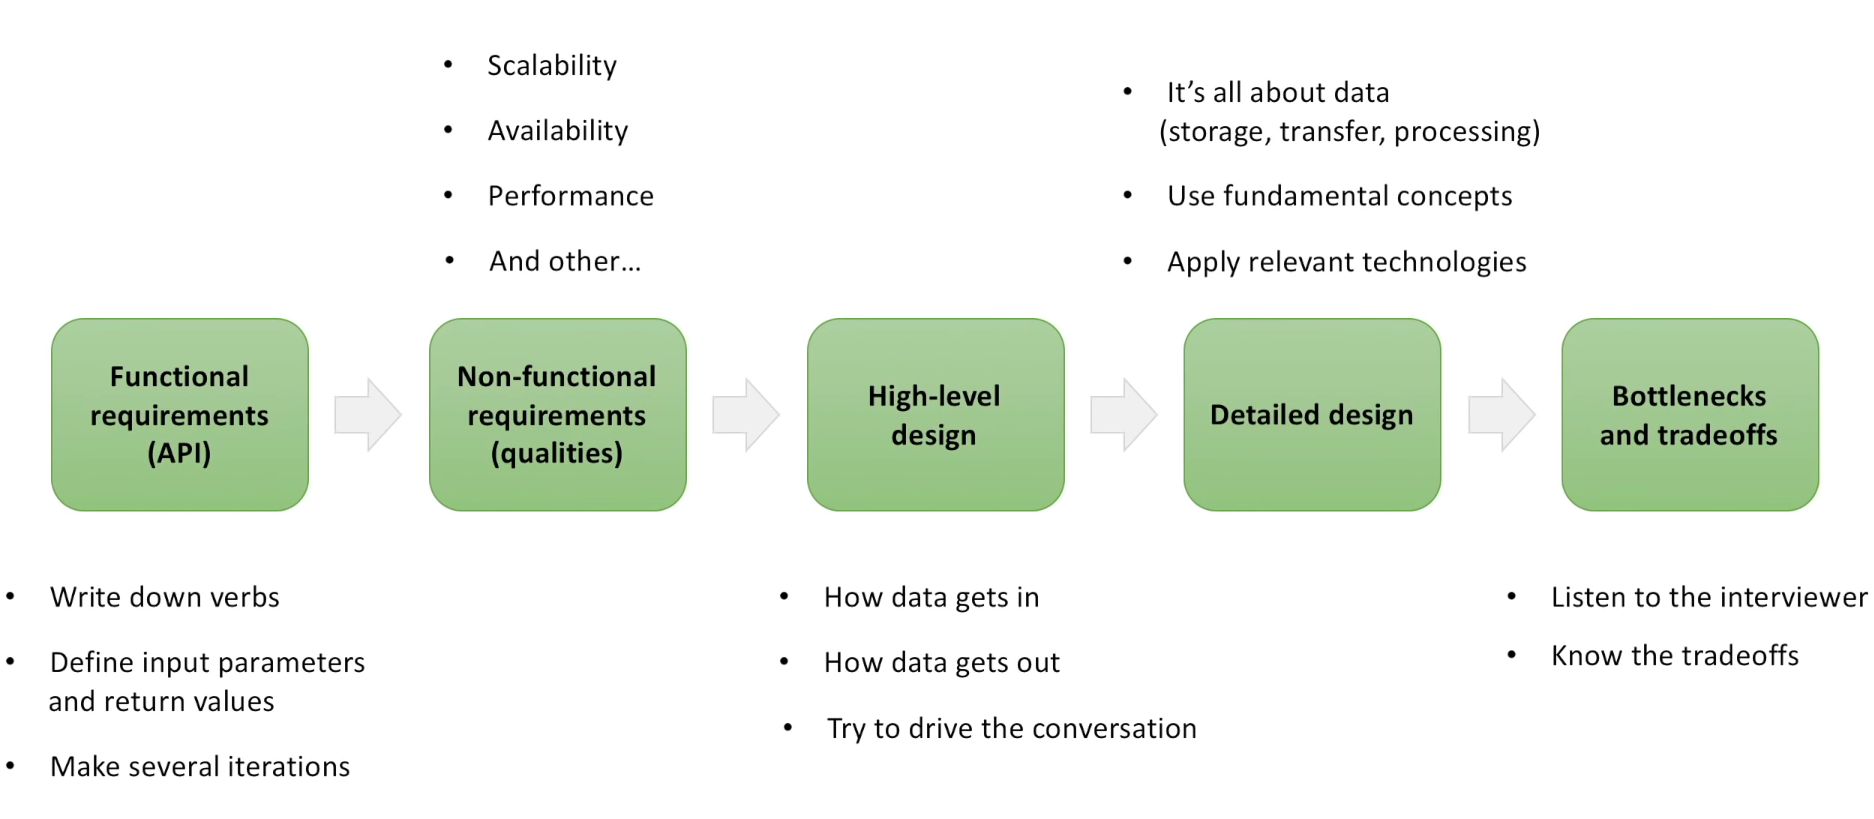
\includegraphics[width=12cm]{assets/system-design-interview.png}
    \caption{Summary of the systems design interview process\cite{sys-design-interview-yt}}
\end{figure}



